% %%%%%%%%%%%%%%%%%%%%%%%%%%%%%%%%%%%%%%%%%%%%%%%%%%%%%
%% 2020 MCM/ICM 模版
%% 本模版根据官方提供的代码优化:http://www.immchallenge.org/mcm/index.html
%% 微信公众号:数学模型(MATHmodels)
%% 联系方式:mathmodels@outlook.com

% %%%%%%%%%%%%%%%%%%%%%%% 说明 %%%%%%%%%%%%%%%%%%%%%%%
%% 本模版将论文的各部分切割成多个 .tex 文件放在 sections 文件
%% 夹中,并用 \input 命令载入到主文档 main.tex 中。
%% 
%% 论文中所用到的图片都放在 figures 文件夹中
%% 
%% 附录中所用到的代码都放在 codes 文件夹中
%%
%% 参考文献按格式整理在 biblo.bib 文本文件中
%%
%% 论文中所有引用链接都有一个彩色框,如果不要,请去将 
%% \usepackage{hyperref} 
%% 替换为
%% \usepackage[hidelinks]{hyperref}
%%
%% 注题:不要忘记更改题号和队号
% %%%%%%%%%%%%%%%%%%%%%%%%%%%%%%%%%%%%%%%%%%%%%%%%%%%%%
\documentclass[12pt]{article}
\usepackage{geometry}
\geometry{left=1in,right=0.75in,top=1in,bottom=1in}
\usepackage{lastpage}
\usepackage{fancyhdr}
\usepackage{color}
\usepackage{longtable}
\usepackage{graphicx}
\usepackage{hyperref} 
% \usepackage[hidelinks]{hyperref}
\usepackage{tabularx}
\usepackage{float}
\usepackage[toc,page,title,titletoc,header]{appendix}
\usepackage[font=small,labelfont=bf]{caption}
\usepackage{graphicx}
\usepackage{ifthen}
\usepackage{tikz}
\usepackage{pgfplots}
\usepackage[framed,numbered,autolinebreaks,useliterate]{mcode}
\usepackage{amsmath,amssymb,amsthm}
\usepackage{graphicx}
\usepackage{xcolor}
\usepackage{fancyhdr}
\usepackage{pgfplots}

% %%%%%%%%%%%%%%%%%%% 题号 & 队号 %%%%%%%%%%%%%%%%%%%%%%
\newcommand{\Problem}{BCF}  % 把 ABCDEF换成你的题号
\newcommand{\Team}{2001234} % 换2001234换成你的队号
% %%%%%%%%%%%%%%%%%%%%%%%%%%%%%%%%%%%%%%%%%%%%%%%%%%%%%

\numberwithin{equation}{section} % 公式编号带小节编号
\graphicspath{{figures/}}        % 设置默认图片路径
\lhead{Team \Team}
\rhead{}
\cfoot{}

\newtheorem{theorem}{Theorem}
\newtheorem{corollary}[theorem]{Corollary}
\newtheorem{lemma}[theorem]{Lemma}
\newtheorem{definition}{Definition}
\pagestyle{fancy}
\rhead{Page \thepage\ of \pageref{LastPage}}
% %%%%%%%%%%%%%%%%%%%%%%%%%%%%%%%%%%%%%%%%%%%%%%%%%%%%%
\begin{document}

\thispagestyle{empty}
\vspace*{-16ex}
\centerline{\begin{tabular}{*3{c}}
	\parbox[t]{0.3\linewidth}{\begin{center}\textbf{Problem Chosen}\\ \Large \textcolor{red}{\Problem}\end{center}}
	& \parbox[t]{0.3\linewidth}{\begin{center}\textbf{2020\\ MCM/ICM\\ Summary Sheet}\end{center}}
	& \parbox[t]{0.3\linewidth}{\begin{center}\textbf{Team Control Number}\\ \Large \textcolor{red}{\Team}\end{center}}	\\
	\hline
\end{tabular}}
% %%%%%%%%%%%%%%%%%%%%%%% 摘要 %%%%%%%%%%%%%%%%%%%%%%%
\begin{center}
\Large\bf Title of you paper   % 论文标题
\end{center}

From here, begin your summary  % 摘要



% %%%%%%%%%%%%%%%%%%%%%%% 目录 %%%%%%%%%%%%%%%%%%%%%%%
\clearpage
\newpage
\setcounter{page}{1}
\tableofcontents\newpage 


% %%%%%%%%%%%%%%%%%%%%%%% 正文 %%%%%%%%%%%%%%%%%%%%%%%
\section{Section example}\label{sec:Section example}

Documents usually have some levels of sections to keep its contents organized. LATEX supports this type of organization and also customization of the sectioning and numbering. The command \textcolor{blue}{\textbackslash section\{ \}} marks the beginning of a new section, inside the braces is set the title. Section numbering is automatic and can be disabled. 

The commands \textcolor{blue}{\textbackslash label} and \textcolor{blue}{\textbackslash ref\{ \}} are used for references. The \textcolor{blue}{\textbackslash label\{ \}} can be set either right before or after the \textcolor{blue}{\textbackslash section} statement. This also works on subsections and subsubsections. For example, section \ref{sec:Section example}.

\section{Citation examples}

BibTeX provides for the storage of all references in an external, flat-file database. (BibLaTeX uses this same syntax.) This database can be referenced in any LaTeX document, and citations made to any record that is contained within the file. This is often more convenient than embedding them at the end of every document written. The BibTeX file for this document is \href{biblo.bib}{biblo.bib}. BibTeX file can be ceated by \href{https://www.zotero.org/}{zotero}.

To actually cite a given document is very easy. Go to the point where you want the citation to appear, and use the following: 
\textcolor{blue}{\textbackslash cite\{keyword\}}, where the \textcolor{blue}{keyword} is that of the bibitem you wish to cite. When LaTeX processes the document, the citation will be cross-referenced with the bibitems and replaced with the appropriate number citation. 

Citation examples: article \cite{Beauregard2005}, book \cite{Hicks2006}, webpage \cite{spotcrime,doboszczak}.

\section{Equation example} \label{sec: equation}

A inline equation is shown as $E = m\cdot c^{2}$, a display equation with number is shown as equation (\ref{eq:EMC})
\begin{equation}\label{eq:EMC}
E = m \cdot c^{2}
\end{equation}
and a display equation without number is shown as follow
\[
E=m\cdot c^{2}
\]

\section{Items example}\label{sec:item}

\begin{itemize}
\item
\item
\item
\end{itemize}

\begin{enumerate}
\item
\item
\item
\end{enumerate}

\section{Table example}\label{sec:table}

A table example is shown as table \ref{tab:Table-example}.

\begin{table}[h]
\centering
\caption{Table example}\label{tab:Table-example}
\begin{tabular}{|c|c|c|c|c|}
\hline 
 & AAAAAA & BBBBBB & CCCCCC & DDDDDD\tabularnewline
\hline 
XXX & 1 & 2 & 3 & 4\tabularnewline
\hline 
YYY & 5 & 6 & 7 & 8\tabularnewline
\hline 
\end{tabular}
\end{table}

\section{Figure example}\label{sec:figure}

A simple figure example is shown as figure \ref{fig:mathmodels}.

\begin{figure}[!htb]
\centering

\includegraphics[width=0.6\textwidth]{MATHmodels.pdf}
\caption{Figure example}\label{fig:mathmodels}
\end{figure}

For two independent side-by-side figures, you can use two minipages inside a figure enviroment. Here's an example, shown as figure \ref{fig:h_example_19} and \ref{fig:h_example_82}.
\begin{figure}[!htb]
\begin{minipage}[t]{0.5\linewidth}
\centering
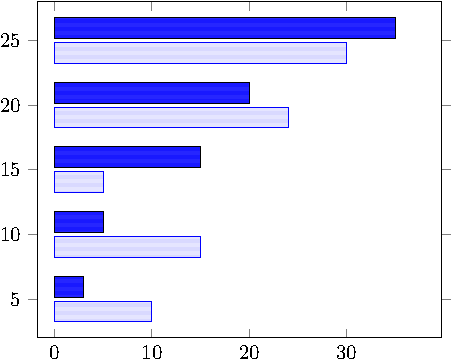
\includegraphics[width=0.8\textwidth]{h_example_19.pdf}
\caption{Figure example}\label{fig:h_example_19}
\end{minipage}
\begin{minipage}[t]{0.5\linewidth}
\centering
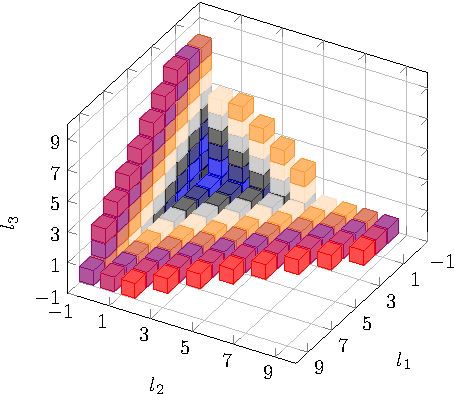
\includegraphics[width=0.8\textwidth]{h_example_82.pdf}
\caption{Figure example}\label{fig:h_example_82}
\end{minipage}
\end{figure}


TikZ and PGF are TeX packages for creating graphics programmatically. TikZ is build on top of PGF and allows you to create sophisticated graphics in a rather intuitive and easy manner. More about tikz, see 
\begin{itemize}
\item TikZ and PGF:  \url{http://www.texample.net/tikz}
\item PGFPlots on Sourceforge:  \url{http://pgfplots.sourceforge.net}
\item PGFPlots examples:  \url{http://pgfplots.net/tikz/examples/}
\end{itemize}
Here are a tikzpicture example (figure \ref{fig:tikz}) and a pgfplots example (figure \ref{fig:pgfplots}).
\begin{figure}[!htb]
\begin{minipage}[t]{0.5\linewidth}
\centering
\usetikzlibrary{arrows,calc,intersections}


\def\r{4}
\def\n{8} \def\myangles{{25,50,85,125,160,220,250,280,340}}
%This vector contains the angles determining the position of the points.
%-----------------------------------------------------------
% Variables and counters used to generate the 4-combinations
\newcounter{np} \pgfmathsetcounter{np}{\n+1}
\newcounter{na} \newcounter{nb} \newcounter{nc}
\newcounter{ia} 
\pgfmathsetcounter{na}{\n-1}    % saves some computations later
\pgfmathsetcounter{nb}{\n-2}    % ""
\pgfmathsetcounter{nc}{\n-3}    %   ""
\newcounter{q} \setcounter{q}{0}    % if flag q=1 then exit the whiledo loop
\newcounter{e} \setcounter{e}{0}    % e counts the combinations!
\newcounter{a} \setcounter{a}{0}    % element of the 4-combination
\newcounter{b} \setcounter{b}{1}    % ""
\newcounter{c} \setcounter{c}{2}    % ""
\newcounter{d} \setcounter{d}{2}    % ""
%Watch out! The initial value {0,1,2,2} is not a 4-combination
\begin{tikzpicture}[scale=0.7,font=\footnotesize]
    % Draw the complete graph
    \fill[fill=blue!10!green!10!,draw=blue,dotted,thick] (0,0) circle (\r);
    \pgfmathparse{\n-1} \let\nn\pgfmathresult 
    \foreach \i in {0,...,\nn}{
        \pgfmathparse{\i+1} \let\ii\pgfmathresult
        \pgfmathparse{\myangles[\i]} \let\t\pgfmathresult
        \foreach \j in {\ii,...,\n}
            \pgfmathparse{\myangles[\j]} \let\u\pgfmathresult
            \draw[blue,very thick] ({\r*cos(\t)},{\r*sin(\t)})--({\r*cos(\u)},{\r*sin(\u)});
        }
    \foreach \i in {0,...,\n}{
        \pgfmathparse{\myangles[\i]}    \let\t\pgfmathresult
        \pgfmathsetcounter{ia}{\i+1}
        \fill[draw=blue,fill=blue!20!,thick]
                ({\r*cos(\t)},{\r*sin(\t)})circle (2.5mm) node{$\mathbf{\theia}$};
        }
        % Points and segments are now drawn
        %
    \whiledo{\theq=0}{ % this loop generates the 4-combinations
        \stepcounter{e}
        \ifthenelse{\thee=1000}{\setcounter{q}{1}}{}% just to be sure to get out of the loop some day...
        \ifthenelse{\thed=\n}
            {\ifthenelse{\thec=\thena}
                {\ifthenelse{\theb=\thenb}
                    {\ifthenelse{\thea=\thenc}
                        {\setcounter{q}{1}}
                        {   \stepcounter{a}
                            \pgfmathsetcounter{b}{\thea+1}
                            \pgfmathsetcounter{c}{\thea+2}
                            \pgfmathsetcounter{d}{\thea+3}                  
                        }
                    }
                    {   \stepcounter{b}
                        \pgfmathsetcounter{c}{\theb+1}
                        \pgfmathsetcounter{d}{\theb+2}                      
                    }
                }
                {   \stepcounter{c}
                    \pgfmathsetcounter{d}{\thec+1}
                }
            }
            {\stepcounter{d}}
        \ifthenelse{\theq=0}{
            % Construction of the intersection points of the segments
            \pgfmathparse{\r*cos(\myangles[\thea])} \let\xa\pgfmathresult
            \pgfmathparse{\r*sin(\myangles[\thea])} \let\ya\pgfmathresult
            \pgfmathparse{\r*cos(\myangles[\theb])} \let\xb\pgfmathresult
            \pgfmathparse{\r*sin(\myangles[\theb])} \let\yb\pgfmathresult
            \pgfmathparse{\r*cos(\myangles[\thec])} \let\xc\pgfmathresult
            \pgfmathparse{\r*sin(\myangles[\thec])} \let\yc\pgfmathresult
            \pgfmathparse{\r*cos(\myangles[\thed])} \let\xd\pgfmathresult
            \pgfmathparse{\r*sin(\myangles[\thed])} \let\yd\pgfmathresult
            %               
            \coordinate  (A) at (\xa,\ya);
            \coordinate  (B) at (\xb,\yb);
            \coordinate  (C) at (\xc,\yc);
            \coordinate  (D) at (\xd,\yd);
            % Name the coordinates, but do not draw anything!               
            \path[name path=sega] (A) -- (C);
            \path[name path=segb] (B) -- (D);
            \path [name intersections={of=sega and segb}];
            \coordinate (X) at (intersection-1);
            \fill[fill=green!50!,draw=blue] (X) circle (0.8mm);             
            %-----------------------------------------------------
            }{}
    }% End of the whiledo loop
\end{tikzpicture}

\caption{tikzpicture example. }\label{fig:tikz}
\end{minipage}
\begin{minipage}[t]{0.5\linewidth}
\centering
\centering
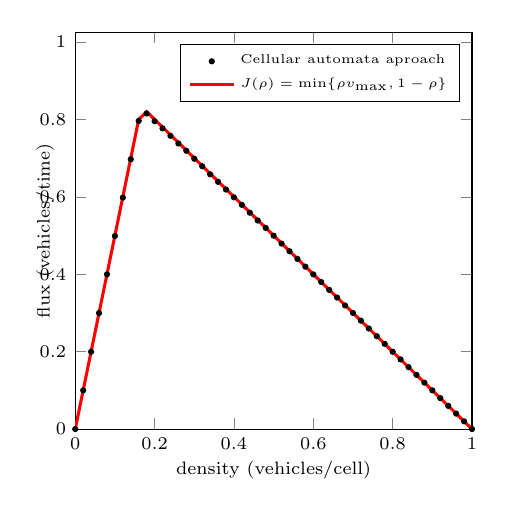
\begin{tikzpicture}[scale=0.925]
	\begin{axis}[xmin=0, xmax=1, ymin=0, ymax=1.025, width=200pt, height=200pt,
xlabel={density (vehicles/cell)},
ylabel={flux (vehicles/time)},
label style={anchor=near ticklabel},
    ylabel style={yshift=-1.25em},
    xlabel style={yshift=0.25em},
    tick label style={font=\scriptsize },
    label style={font=\scriptsize},
legend style={font=\tiny,legend cell align=left,legend pos=north east}
]
	\addplot[only marks, mark size=1]%
	table[x=rho,y=pridict] {
      rho        pridict       theory
         0         0         0
    0.0200    0.1000    0.1000
    0.0400    0.1998    0.2000
    0.0600    0.2998    0.3000
    0.0800    0.3996    0.4000
    0.1000    0.4988    0.5000
    0.1200    0.5980    0.6000
    0.1400    0.6970    0.7000
    0.1600    0.7960    0.8000
    0.1800    0.8152    0.8200
    0.2000    0.7954    0.8000
    0.2200    0.7768    0.7800
    0.2400    0.7576    0.7600
    0.2600    0.7378    0.7400
    0.2800    0.7190    0.7200
    0.3000    0.6984    0.7000
    0.3200    0.6790    0.6800
    0.3400    0.6582    0.6600
    0.3600    0.6388    0.6400
    0.3800    0.6188    0.6200
    0.4000    0.5986    0.6000
    0.4200    0.5792    0.5800
    0.4400    0.5590    0.5600
    0.4600    0.5388    0.5400
    0.4800    0.5196    0.5200
    0.5000    0.4996    0.5000
    0.5200    0.4792    0.4800
    0.5400    0.4594    0.4600
    0.5600    0.4396    0.4400
    0.5800    0.4196    0.4200
    0.6000    0.3996    0.4000
    0.6200    0.3798    0.3800
    0.6400    0.3596    0.3600
    0.6600    0.3398    0.3400
    0.6800    0.3194    0.3200
    0.7000    0.3000    0.3000
    0.7200    0.2800    0.2800
    0.7400    0.2598    0.2600
    0.7600    0.2400    0.2400
    0.7800    0.2200    0.2200
    0.8000    0.1998    0.2000
    0.8200    0.1800    0.1800
    0.8400    0.1600    0.1600
    0.8600    0.1400    0.1400
    0.8800    0.1200    0.1200
    0.9000    0.1000    0.1000
    0.9200    0.0800    0.0800
    0.9400    0.0600    0.0600
    0.9600    0.0400    0.0400
    0.9800    0.0200    0.0200
    1.0000         0         0
	};
\addlegendentry{Cellular automata aproach}
	\addplot[mark=none, red, very thick]%
	table[x=rho,y=theory] {
      rho        pridict       theory
         0         0         0
    0.0200    0.1000    0.1000
    0.0400    0.1998    0.2000
    0.0600    0.2998    0.3000
    0.0800    0.3996    0.4000
    0.1000    0.4988    0.5000
    0.1200    0.5980    0.6000
    0.1400    0.6970    0.7000
    0.1600    0.7960    0.8000
    0.1800    0.8152    0.8200
    0.2000    0.7954    0.8000
    0.2200    0.7768    0.7800
    0.2400    0.7576    0.7600
    0.2600    0.7378    0.7400
    0.2800    0.7190    0.7200
    0.3000    0.6984    0.7000
    0.3200    0.6790    0.6800
    0.3400    0.6582    0.6600
    0.3600    0.6388    0.6400
    0.3800    0.6188    0.6200
    0.4000    0.5986    0.6000
    0.4200    0.5792    0.5800
    0.4400    0.5590    0.5600
    0.4600    0.5388    0.5400
    0.4800    0.5196    0.5200
    0.5000    0.4996    0.5000
    0.5200    0.4792    0.4800
    0.5400    0.4594    0.4600
    0.5600    0.4396    0.4400
    0.5800    0.4196    0.4200
    0.6000    0.3996    0.4000
    0.6200    0.3798    0.3800
    0.6400    0.3596    0.3600
    0.6600    0.3398    0.3400
    0.6800    0.3194    0.3200
    0.7000    0.3000    0.3000
    0.7200    0.2800    0.2800
    0.7400    0.2598    0.2600
    0.7600    0.2400    0.2400
    0.7800    0.2200    0.2200
    0.8000    0.1998    0.2000
    0.8200    0.1800    0.1800
    0.8400    0.1600    0.1600
    0.8600    0.1400    0.1400
    0.8800    0.1200    0.1200
    0.9000    0.1000    0.1000
    0.9200    0.0800    0.0800
    0.9400    0.0600    0.0600
    0.9600    0.0400    0.0400
    0.9800    0.0200    0.0200
    1.0000         0         0
	};
\addlegendentry{$J(\rho) = \min\{\rho v_{\max}, 1-\rho\}$}
\end{axis}
\end{tikzpicture}

\caption{pgfplots example}\label{fig:pgfplots}
\end{minipage}
\end{figure}



% %%%%%%%%%%%%%%%%%%%%% 参考文献 %%%%%%%%%%%%%%%%%%%%%
\newpage
\bibliographystyle{unsrt}
\bibliography{biblo}
\newpage


% %%%%%%%%%%%%%%%%%%%%%%% 附录 %%%%%%%%%%%%%%%%%%%%%%%% 
\appendixpage
\appendix

\section{Your First Appendix}

From here, begin your first Appdendix... your can include some program
script, such as matlab, c/cpp, python.

\subsection{MATLAB example}
\lstinputlisting{codes/example.m}


% ------------------------------------------------------------------------

\section{Your Second Appendix}
\begin{longtable}{c|c|c}
\caption{Data example(Here we use long table)}\\
\hline 
AAAAAAAAAAAAAAAAA & BBBBBBBBBBBBBBBBB & CCCCCCCCCCCCCCCCC\\
\endfirsthead
\hline 
AAAAAAAAAAAAAAAAA & BBBBBBBBBBBBBBBBB & CCCCCCCCCCCCCCCCC\\
\hline 
\endhead
\hline 
 1 &  & \\
 2 &  & \\
 3 &  & \\
 4 &  & \\
 5 &  & \\      \hline 
 6 &  & \\
 7 &  & \\
 8 &  & \\
 9 &  & \\
10 &  & \\     \hline 
11 &  & \\
12 &  & \\
13 &  & \\
14 &  & \\
15 &  & \\     \hline 
16 &  & \\
17 &  & \\
18 &  & \\
19 &  & \\
20 &  & \\
\hline 
\end{longtable}


\end{document}
